% =====================================================================================
%  Section 4.3 — Can the shield's safety be internalised?
%  Self-contained. Nothing to \input.
%
%  PREAMBLE (all already in main.tex): graphicx, booktabs, multirow, threeparttable
%  Additionally requires \usepackage{siunitx} ONLY if you switch to S columns; not used here.
%
%  ASSET: figures/fig_internalisation.pdf
%    Regenerate:  PYTHONPATH=. python -m experiments.make_fig_internalisation
%
%  STILL TO MAKE: Figure 4.3, the qualitative filmstrip. See the commented block at the end of
%  this file -- it cannot be built until the source episodes are identified.
%
%  NUMBER PROVENANCE: figures/results_shielded_distillation.md, eval 2026-08-07,
%  held-out inits 35-39, n = 120 per condition, 24 scenes.
% =====================================================================================

\section{Can the Shield's Safety Be Internalised?}\label{sec:res:internalise}

A runtime filter must run forever. It occupies inference budget on every control step, requires
obstacle geometry at deployment, and is a component that can fail. The central question of this
work is whether the behaviour it induces can instead be absorbed into the policy, so that the
policy is safe with the filter switched off.

Demonstrations were collected by rolling out the shielded policy and retaining episodes that
succeeded, displaced nothing, and in which the shield actually intervened at least once. That last
criterion matters: a clean episode in which the shield never fired is ordinary base-policy
behaviour and teaches nothing about safety. The retained set was 186 demonstrations from 480
rollouts, a 39\% yield. These were behaviour-cloned into the policy's action head, and the
procedure was repeated for a second round.

\begin{figure}[htbp]
  \centering
  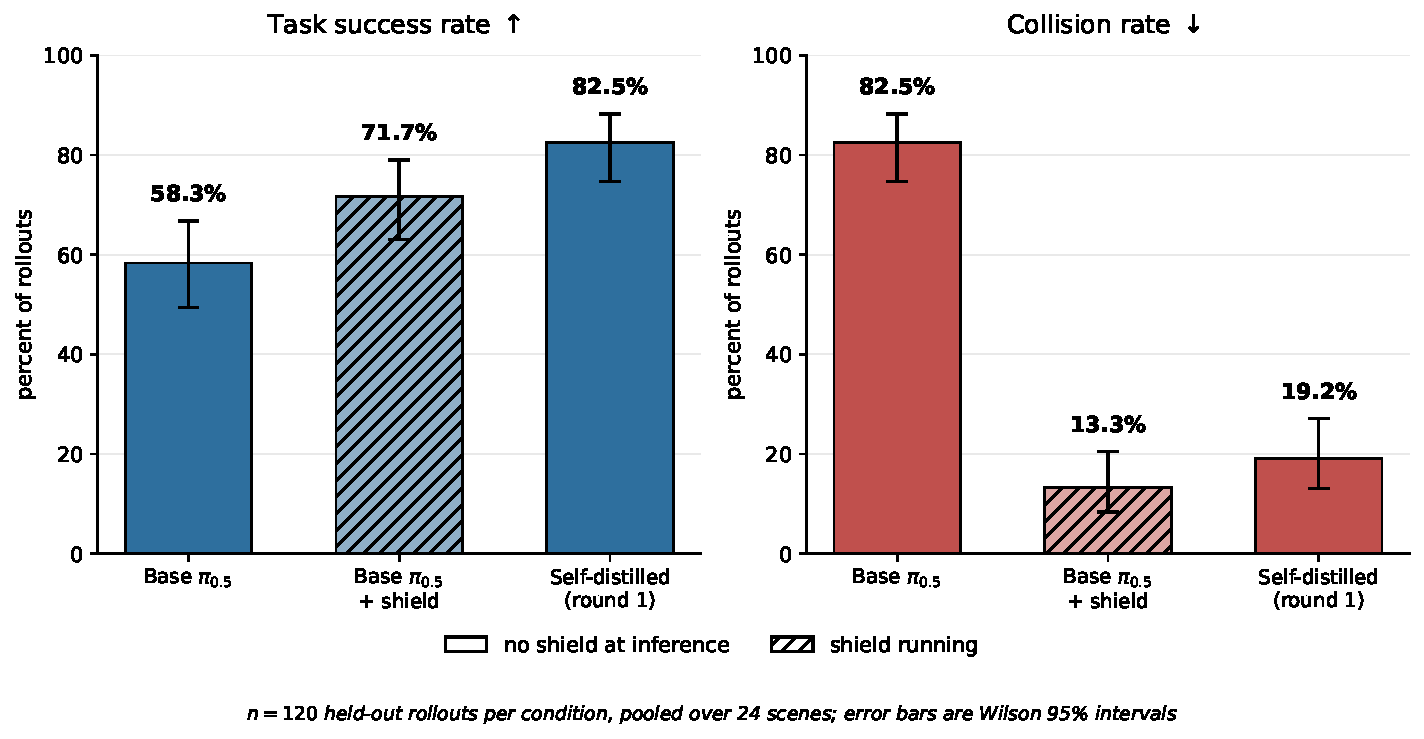
\includegraphics[width=\linewidth]{figures/fig_internalisation.pdf}
  \caption[Internalisation of the shield's safety]{%
    The central result. The self-distilled policy, running with \emph{no shield at inference}
    (solid), is both safer and more successful than the base policy it was distilled from, and
    recovers most of the safety of the shielded baseline (hatched). Error bars are Wilson 95\%
    intervals at $n = 120$ held-out rollouts per condition.}
  \label{fig:internalisation}
\end{figure}

\begin{table}[htbp]
\centering
\begin{threeparttable}
\caption[Effect of self-distillation on safety and task performance]{%
  Effect of self-distillation, with and without the shield at inference. Rows in bold are the
  shield-free distilled policies, which are the claim of this work. $n = 120$ held-out rollouts
  per row, pooled over 24 scenes; intervals are Wilson 95\%.}
\label{tab:internalisation}
\begin{tabular}{lcccrr}
\toprule
\textbf{Policy} & \textbf{TSR (95\% CI)} & \textbf{Collision (95\% CI)} & \textbf{CAR}
  & $\lvert r_{\mathrm{cbf}}\rvert$\tnote{a} & \textbf{ETS}\tnote{b} \\
\midrule
Base, no shield        & 58.3\% [49.4, 66.8] & 82.5\% [74.7, 88.3] & 17.5\% & ---   & 138.6 \\
Base + shield          & 71.7\% [63.0, 79.0] & 13.3\% [\phantom{0}8.4, 20.6] & 86.7\% & 0.533 & 160.6 \\
\addlinespace[3pt]
\textbf{Round 1, no shield} & \textbf{82.5\% [74.7, 88.3]} & \textbf{19.2\% [13.1, 27.1]}
  & \textbf{80.8\%} & --- & 157.3 \\
Round 1 + shield       & 70.8\% [62.2, 78.2] & \phantom{0}8.3\% [\phantom{0}4.6, 14.7] & 91.7\% & 0.265 & 170.0 \\
\addlinespace[3pt]
\textbf{Round 2, no shield} & \textbf{80.8\% [72.9, 86.9]} & \textbf{17.5\% [11.7, 25.3]}
  & \textbf{82.5\%} & --- & 158.8 \\
Round 2 + shield       & 72.5\% [63.9, 79.7] & \phantom{0}9.2\% [\phantom{0}5.2, 15.7] & 90.8\% & 0.273 & 176.7 \\
\bottomrule
\end{tabular}
\begin{tablenotes}[flushleft]\footnotesize
\item[a] Mean absolute CBF reward term, a proxy for how much the shield had to correct. Necessarily
  zero when no shield is running, shown as ---.
\item[b] Execution time to success, in control steps, over successful rollouts only
  (Section~\ref{sec:metrics}). Conditional on success and must be read alongside TSR.
\end{tablenotes}
\end{threeparttable}
\end{table}

The headline result is the third row. With no shield running at inference, the distilled policy
displaces the obstacle in 19.2\% of episodes, against 82.5\% for the policy it was distilled
from~--- and its success rate rises from 58.3\% to 82.5\%. Both intervals are disjoint from the
base policy's. The distilled policy is simultaneously safer and more capable than its own teacher,
without the teacher's filter.

It is worth noting how close this comes to the shielded baseline: CAR 80.8\% shield-free against
86.7\% with the shield active. Most of the shield's safety benefit survives its removal.

\paragraph{One round is enough.}
Rounds one and two overlap on both metrics, so the second round buys nothing measurable. It also
does not erode performance, which is worth stating explicitly: an earlier DAgger-style experiment
in this project degraded across rounds (Section~\ref{sec:res:source}), and the absence of that
degradation here is informative rather than merely convenient.

\paragraph{Stacking the shield costs success.}
Applying the shield to the distilled policy improves safety further (CAR 80.8\% to 91.7\%) but
reduces success (82.5\% to 70.8\%). This is the mirror image of Section~\ref{sec:shield_efficacy}
and has the same explanation. The shield operates by projecting the policy's action onto the safe
set. When the policy frequently proposes unsafe actions, that projection is a net benefit. When the
policy already avoids the obstacle, the projection instead perturbs actions that were already both
safe and competent, displacing them from the distribution the policy was trained to produce~---
safe, but no longer a well-formed grasp. The claim of this work is therefore about shield-free
operation, not about stacking the two.

\paragraph{The cost of internalised caution.}
ETS rises from 138.6 to 157.3 steps, roughly 14\% slower. The distilled policy takes a more
conservative route. This is a real cost and is reported rather than omitted.

\paragraph{Characterising the training data.}
Because the demonstrations are the mechanism, their content is worth quantifying. Across the 186
retained demonstrations the shield was active on a median of 32\% of control steps, with a median
of 51 activations per episode, a minimum of nine, and no demonstration below five. The mean
correction norm was 0.33 against actions bounded at $\pm 1$ per axis. Roughly one imitated action
in three was therefore modified by the barrier, and modified substantially: the imitated action
distribution differs materially from the base policy's own.

% =====================================================================================
%  FIGURE 4.3 — qualitative filmstrip.  NOT YET BUILDABLE.
%
%  Intent: same scene and same held-out initial state, base pi0.5 (collides) above and the
%  distilled policy (avoids) below, 4-5 frames each, contact frame boxed or arrowed. Every other
%  figure in this chapter reports a rate; none shows the behaviour, so this is the largest
%  qualitative gain available to the chapter.
%
%  BLOCKED ON: videos/ contains task3_ep0.mp4, task3_ep1.mp4, task3_ep3.mp4 with no record of
%  which policy produced them, which scene they are, or whether any contains a collision. Pairing
%  them by guesswork would risk captioning a distilled rollout as the base policy.
%
%  TO UNBLOCK, record for two rollouts of the SAME scene and SAME held-out init:
%    (i) base policy, an episode that collides;  (ii) round-1 distilled, an episode that does not.
%  Then:  PYTHONPATH=. python -m experiments.make_fig_filmstrip \
%             --base <base.mp4> --distilled <distilled.mp4> --contact-frame <N>
%  (that script does not exist yet either -- write it once the inputs are known.)
%
%  \begin{figure}[htbp]
%    \centering
%    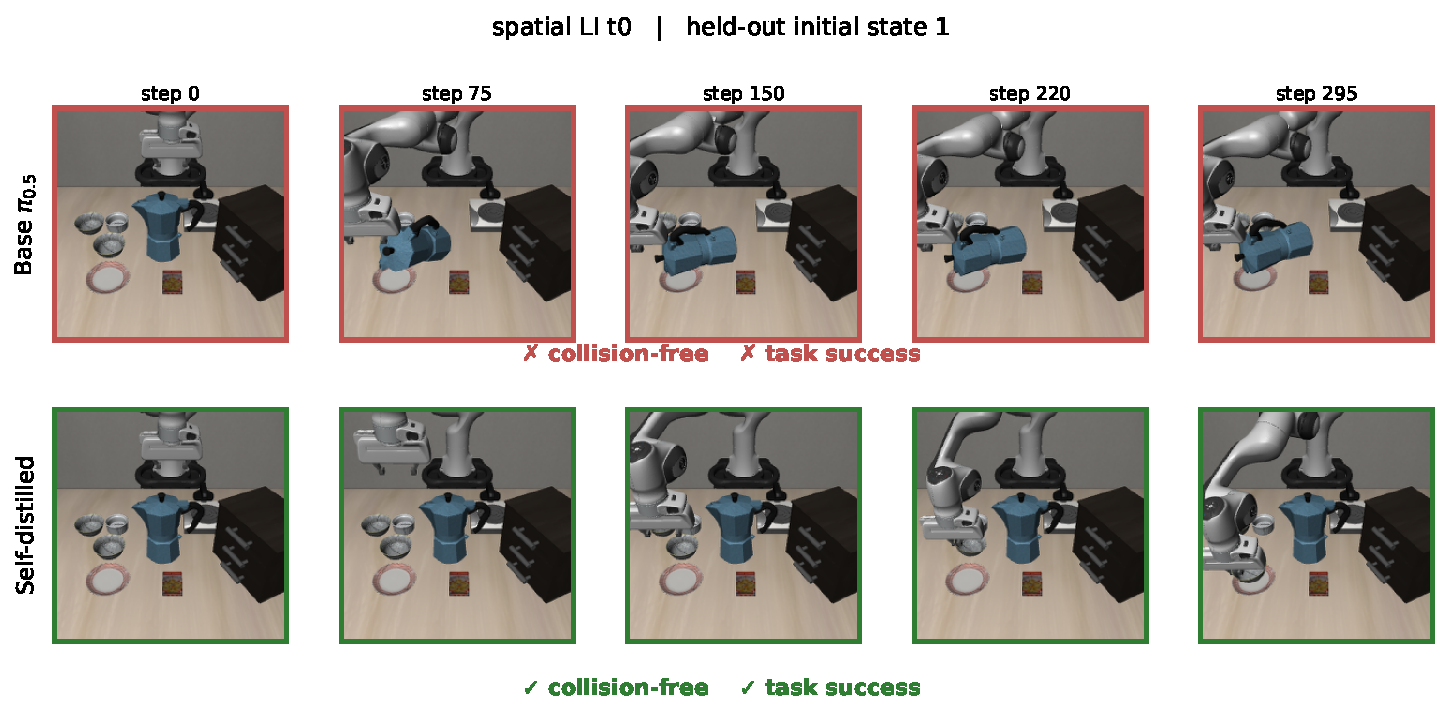
\includegraphics[width=\linewidth]{figures/fig_filmstrip.pdf}
%    \caption{...}
%    \label{fig:filmstrip}
%  \end{figure}
% =====================================================================================
